% !TeX program = pdflatex
% !TeX root = GSE.tex

\documentclass[../FeynCalcManual.tex]{subfiles}
\begin{document}
\hypertarget{gse}{%
\section{GSE}\label{gse}}

\texttt{GSE[\allowbreak{}p]} can be used as input for a
\(D-4\)-dimensional \(\gamma \cdot p = \gamma^\mu p_\mu\) and is
transformed into
\texttt{DiracGamma[\allowbreak{}Momentum[\allowbreak{}p,\ \allowbreak{}D-4],\ \allowbreak{}D-4]}
by \texttt{FeynCalcInternal} (\texttt{FCI}).
\texttt{GSE[\allowbreak{}p,\ \allowbreak{}q,\ \allowbreak{}...]} is a
short form for \texttt{GSE[\allowbreak{}p].GSE[\allowbreak{}q]. ...}.

\subsection{See also}

\hyperlink{toc}{Overview}, \hyperlink{diracgamma}{DiracGamma},
\hyperlink{ga}{GA}, \hyperlink{gad}{GAD}, \hyperlink{gsd}{GSD}.

\subsection{Examples}

\begin{Shaded}
\begin{Highlighting}[]
\NormalTok{GSE}\OperatorTok{[}\FunctionTok{p}\OperatorTok{]}
\end{Highlighting}
\end{Shaded}

\begin{dmath*}\breakingcomma
\hat{\gamma }\cdot \hat{p}
\end{dmath*}

\begin{Shaded}
\begin{Highlighting}[]
\NormalTok{GSE}\OperatorTok{[}\FunctionTok{p}\OperatorTok{]} \SpecialCharTok{//}\NormalTok{ FCI }\SpecialCharTok{//} \FunctionTok{StandardForm}

\CommentTok{(*DiracGamma[Momentum[p, {-}4 + D], {-}4 + D]*)}
\end{Highlighting}
\end{Shaded}

\begin{Shaded}
\begin{Highlighting}[]
\NormalTok{GSE}\OperatorTok{[}\FunctionTok{p}\OperatorTok{,} \FunctionTok{q}\OperatorTok{,} \FunctionTok{r}\OperatorTok{,} \FunctionTok{s}\OperatorTok{]}
\end{Highlighting}
\end{Shaded}

\begin{dmath*}\breakingcomma
\left(\hat{\gamma }\cdot \hat{p}\right).\left(\hat{\gamma }\cdot \hat{q}\right).\left(\hat{\gamma }\cdot \hat{r}\right).\left(\hat{\gamma }\cdot \hat{s}\right)
\end{dmath*}

\begin{Shaded}
\begin{Highlighting}[]
\NormalTok{GSE}\OperatorTok{[}\FunctionTok{p}\OperatorTok{,} \FunctionTok{q}\OperatorTok{,} \FunctionTok{r}\OperatorTok{,} \FunctionTok{s}\OperatorTok{]} \SpecialCharTok{//} \FunctionTok{StandardForm}

\CommentTok{(*GSE[p] . GSE[q] . GSE[r] . GSE[s]*)}
\end{Highlighting}
\end{Shaded}

\begin{Shaded}
\begin{Highlighting}[]
\NormalTok{GSE}\OperatorTok{[}\FunctionTok{q}\OperatorTok{]}\NormalTok{ . (GSE}\OperatorTok{[}\FunctionTok{p}\OperatorTok{]} \SpecialCharTok{+} \FunctionTok{m}\NormalTok{) . GSE}\OperatorTok{[}\FunctionTok{q}\OperatorTok{]}
\end{Highlighting}
\end{Shaded}

\begin{dmath*}\breakingcomma
\left(\hat{\gamma }\cdot \hat{q}\right).\left(m+\hat{\gamma }\cdot \hat{p}\right).\left(\hat{\gamma }\cdot \hat{q}\right)
\end{dmath*}

In order to use Dirac algebra with \(D-4\) dimensional objects you need
to activate the t'Hooft-Veltman-Breitenlohner-Maison scheme first

\begin{Shaded}
\begin{Highlighting}[]
\NormalTok{FCSetDiracGammaScheme}\OperatorTok{[}\StringTok{"NDR"}\OperatorTok{]}\NormalTok{; }
 
\NormalTok{DiracSimplify}\OperatorTok{[}\NormalTok{GSE}\OperatorTok{[}\FunctionTok{q}\OperatorTok{]}\NormalTok{ . GS}\OperatorTok{[}\FunctionTok{q}\OperatorTok{]}\NormalTok{ . GSE}\OperatorTok{[}\FunctionTok{q}\OperatorTok{]]}
\end{Highlighting}
\end{Shaded}

\begin{figure}[!ht]
\centering
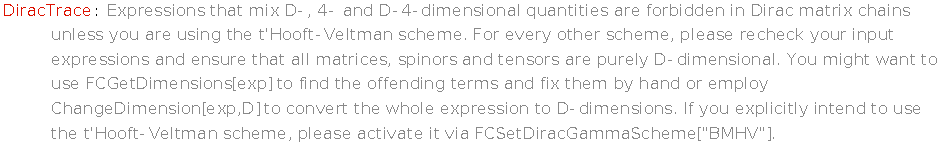
\includegraphics[width=0.6\linewidth]{img/1h0chl63b60ya.pdf}
\end{figure}

\begin{dmath*}\breakingcomma
\text{\$Aborted}
\end{dmath*}

\begin{Shaded}
\begin{Highlighting}[]
\NormalTok{FCSetDiracGammaScheme}\OperatorTok{[}\StringTok{"BMHV"}\OperatorTok{]}\NormalTok{; }
 
\NormalTok{DiracSimplify}\OperatorTok{[}\NormalTok{GSE}\OperatorTok{[}\FunctionTok{q}\OperatorTok{]}\NormalTok{ . GS}\OperatorTok{[}\FunctionTok{q}\OperatorTok{]}\NormalTok{ . GSE}\OperatorTok{[}\FunctionTok{q}\OperatorTok{]]}
\end{Highlighting}
\end{Shaded}

\begin{dmath*}\breakingcomma
\hat{q}^2 \left(-\left(\bar{\gamma }\cdot \overline{q}\right)\right)
\end{dmath*}

\begin{Shaded}
\begin{Highlighting}[]
\NormalTok{FCSetDiracGammaScheme}\OperatorTok{[}\StringTok{"NDR"}\OperatorTok{]}\NormalTok{;}
\end{Highlighting}
\end{Shaded}

\end{document}
